\begin{figure}[!ht]
	\begin{center}
		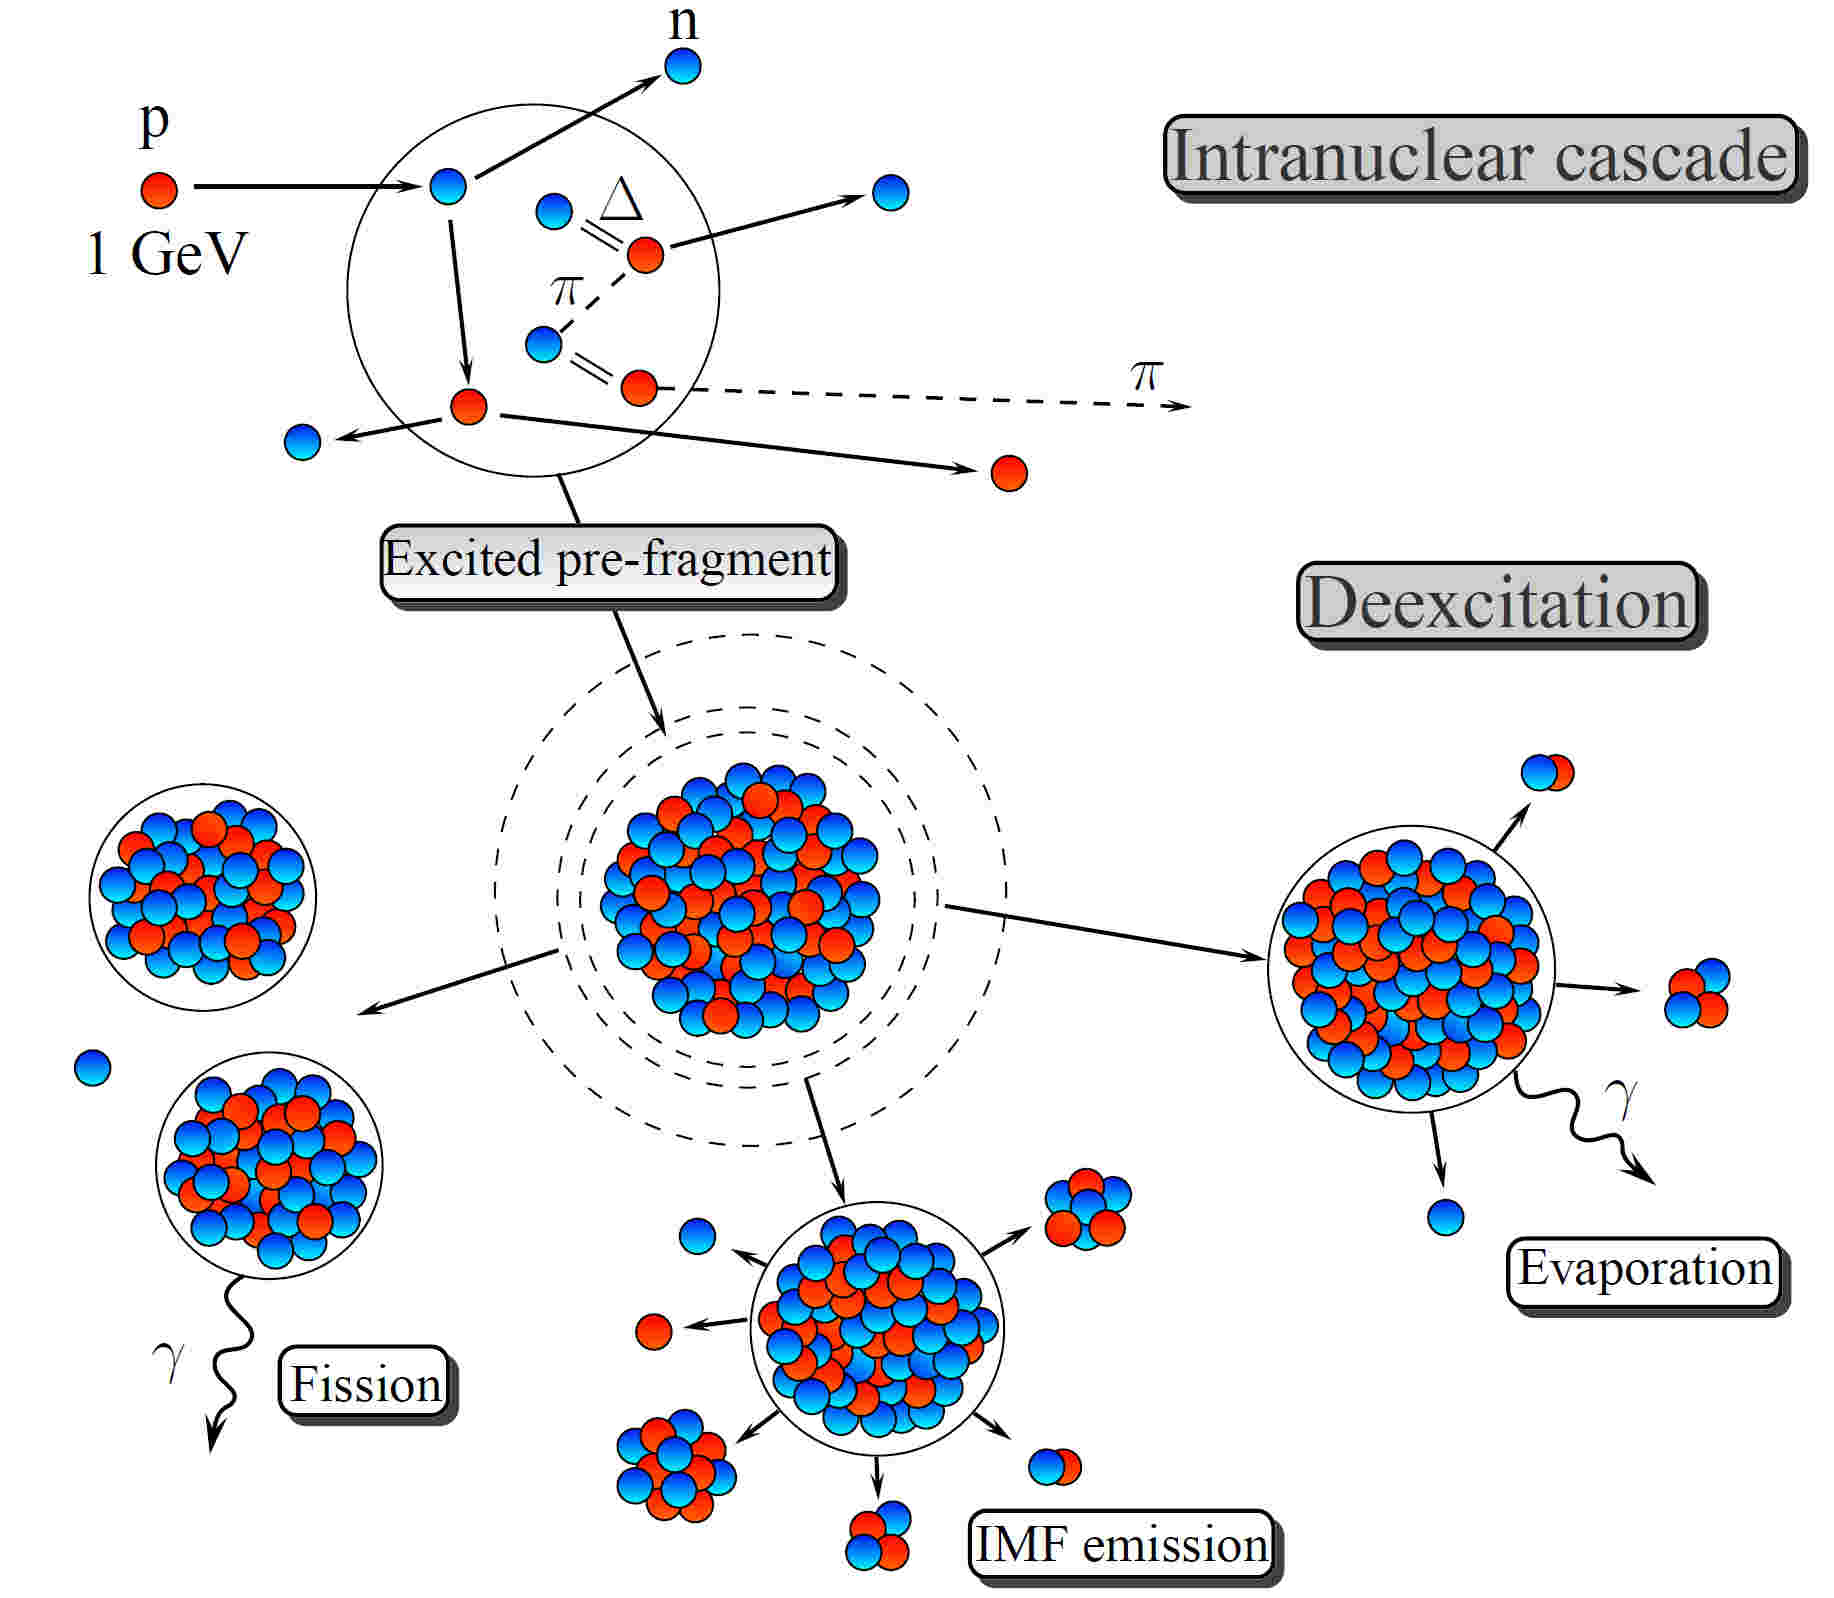
\includegraphics[width=0.8\textwidth]{01_Introduction/figures/fig000_spallation}
	\end{center}
	\caption[Schematic view of the spallation process]{Schematic view of the spallation process \cite{gorbinet:tel-00660583}. The incident protons interact with nucleons of the target. An intranuclear cascade occurs leaving the target atom in an excited state. Depending on the properties of the excited nucleus, different de-excitation process may occur. IMF stands for intermediate mass fragment.}
	\label{chap1:fig:spallation}
\end{figure}
